\documentclass[a4paper,10pt]{report}
\usepackage[utf8]{inputenc}
\usepackage[T1]{fontenc}
\usepackage[francais]{babel}
\usepackage{graphicx} 
\usepackage{enumitem}
\usepackage{underscore}
\usepackage{float}
\usepackage{array}
\usepackage{geometry}
\usepackage{titlesec} 
\usepackage{titletoc}
\usepackage{vmargin}
\usepackage{fancyhdr}

\makeatletter

\setlength{\headheight}{11.0pt}

\renewcommand{\headrulewidth}{1pt}

\titlespacing*{\chapter}
  {0pt}		% retrait à gauche
  {0pt}		% espace avant
  {30pt}	% espace après
   [0pt]	% retrait à droite
   
% Style du titre de chapitre
\titleformat{\chapter}[frame]{\huge\normalfont\sc}{\filright\footnotesize\enspace CHAPITRE \thechapter\enspace}{8pt}{\filcenter}{}
  
  
% Style de titre de section
%\titleformat{\section}[hang]{\bfseries\sc}{\Large\thesection}{1em}{}


% Mise en place du Sommaire
\titlecontents{chapter}[3em]{\addvspace{1em plus 0pt}\bfseries\Large}{\contentslabel{2em}}{\hspace{-1.3em}}{\hfill\contentspage}[\addvspace{3pt}]

% Title Page
\begin{titlepage}

\title{Master 1 Bioinformatique\\Stat'n Dat}


\author{DAHMANI Amal\\JAMART Kevin\\LOPEZ Myriam\\\\}

\end{titlepage}


\begin{document}

\renewcommand{\contentsname}{Sommaire}


\maketitle
\newpage
\tableofcontents
\addtocontents{toc}{\protect\thispagestyle{empty} 
                    \protect\pagestyle{empty}}
\setcounter{tocdepth}{3}     % Dans la table des matieres
\setcounter{secnumdepth}{3}  % Avec un numero.


\newpage
\thispagestyle{empty}
\setcounter{page}{1}
\addcontentsline{toc}{section}{Introduction}

\chapter*{Introduction}


 
\chapter{Analyse}

\section{Etat de l'existant}

En vue de pouvoir répondre à la problématique initiale, nous avons étudié les avantages et inconvénients de quelques logiciels déjà existants.

\subsection{SAS-Statistical Analysis System}
SAS est un logiciel portable complet qui couvre une large gamme des méthodes d’analyse en statistique. Se présentant sous la forme d’un ensemble de modules adaptés pour la gestion de données et l’analyse statistique, il permet de prendre en charge des volumes de données très importants, de l’ordre de plusieurs Go. \\
	Il permet également la création de tableaux de bord KPI et donne la possibilité de programmer ses propres procédures ainsi qu’automatiser l’enchaînement de plusieurs traitements. \\
	Les tableaux de bord KPI ont pour but de représenter sur un page un indicateur clé du suivi de l’activité d’une société. \\

Au contraire, SAS étant un logiciel propriétaire et payant, il est connu pour son coût élevé d’une valeur de 2000 à 5000 \euro en fonction des éditions, pour les professionnels de l’industrie. Son coût est réduit pour les enseignants de l’Académie et il est gratuit pour les étudiants.\\
Par ailleurs, son langage est peu avancé puisqu’il correspond en fait à une combinaison de plusieurs autres langages de programmation tels que IML ou SQL.
De plus, ce logiciel, qui reste propriétaire, n'est pas open source.
\\

\subsection{SPSS Amos}
Le logiciel AMOS (Analyse of Moment Structure) est un programme visuel qui utilise une interface clic-boutons. Il permet à des débutants qui ne connaissent pas le code informatique, de faire de la modélisation d’équations structurelles. \\

Grâce à l’interface graphique de ce logiciel, couplé à la prise en charge des variables latentes, il est possible d’ajuster son modèle et d’en faire une impression de haute qualité. \\

Parmi ses nombreux autres avantages, ce logiciel portable est également capable d’effectuer un traitement dit FIML pour Full Information Maximum Likelihood qui permet d’analyser, sans biais, des données même incomplètes. De même, il propose un florilège de tests parmi lesquels des tests de normalité multivariée, le maximum de vraisemblance, le bootstrap, la simulation de Monte Carlo etc. \\

Cependant, ce logiciel reste payant, tout comme ses multiples extensions qui ne sont pas fournies avec.  \\

\subsection{SosStat}
SosStats se présente sous la forme d’un tableur, dédié aux professionnels de l’industrie qui ont peu ou pas vraiment d’expérience dans les statistiques. \\

Parmi ses différentes fonctionnalités, son interface propose une zone dite de « projet » qui permet à l’utilisateur de visualiser la liste des analyses déjà effectuées avec le logiciel et permet à l’utilisateur de changer la langue s’il le souhaite.\\
La quantité de données traitées ne dépend que la mémoire de l’ordinateur hôte, ce qui peut être utilise lorsque l’on est face à des giga octets de données. \\
Les fonctionnalités proposées donnent la possibilité de faire toutes sortes d’analyses telles que des statistiques descriptives (histogramme ; boxplot ; matrice de corrélation ou détermination des paramètres de population), des tests de normalité (Kolmogorov ; Anderson Darling ; Shapiro-Wilk), des tests paramétriques ou non, des tests de proportions ou d’équivalence ainsi que des calculs de régression.\\


Cependant, SosStat a un coût, même si celui-ci reste relativement faible comparé aux autres logiciels et l’import depuis une base de donnée ne concerne que les SGBD ODBC, SQLite et MySQL.\\
Ce logiciel est par ailleurs non portable puisqu’il n’est actuellement disponible que pour les plate-forme Unix 64 bits et Windows 32 ou 64 bits.

\subsection{Stata}

Stata est un logiciel de statistiques et d’économétrie largement utilisé par les économistes et les épidémiologistes. Il est également utilisé par la communauté scientifique pour les recherches en médecine et biologie.\\

Une des particularités de Stata par rapport à ses concurrents réside dans son développement guidé par les utilisateurs eux-mêmes. Il repose sur un noyau compilé qui comprend les principales instructions et qui peut éventuellement appeler des procédures annexes livrées en standard ou à télécharger sur les sites miroirs de Stata.\\ 
Le programme est écrit en langage Stata, et les applicatifs sont développés par StataCorp ainsi que par les programmeurs enseignants, étudiants ou scientifiques. D'ailleurs, les packages sont our la plupart codés par la communauté des utilisateurs. \\

Stata sert non seulement d’outil pour les statistiques, mais il sert également de générateur de graphiques, et de puissant gestionnaire de données. En effet, il permet de combiner et remodeler les ensembles de données. 
Enfin, cet outil permet la modification et l'export des graphiques créés, en ESP ou TIF pour la publication, en PNG pour le web, ou en PDF pour la visualisation.\\

Néanmoins, Stata reste payant, avec un coût relativement élevé.\\

Tous ces logiciels très avancés sont malheureusement payants et non open source pour la plupart, ce qui ne nous permet pas de les reprendre te de les améliorer en vue des objectifs de notre clients. D’ailleurs la combinaison de langages informatique dont SAS fait l’objet renforce cette difficulté et la rend présente même si le logiciel était à l’heure actuelle open-source.\\

De même, leurs fonctionnalités restent trop précises et trop nombreuses pour ce dont nous avons besoin, ce qui implique donc des logiciels parfois trop compliqués pour la manipulation ou la modification. \\

Les tableaux de bord KPI de SAS sont certes intéressants pour une entreprise de taille importante qui doit quotidiennement rendre compte de ses résultats techniques, mais cette fonctionnalité reste sans intérêt dans notre cas puisqu’il n’y a pas lieu d’évaluer une quelconque rentabilité.\\

De même, le logiciel AMOS semble plutôt avoir été conçu pour pouvoir effectuer des statistiques de grande envergure dans le cadre d’une étude poussée, faisant intervenir des modèles d’évolution complexes.\\

Finalement, il nous faudrait un logiciel pratique d’utilisation, qui propose un moyen simple et efficace de sélectionner ses données, des statistiques de routines et un accès facile à la représentation visuelle des données. C’est aussi la raison pour laquelle nous souhaitons développer par nous-même l’outil idéal pour notre client.

\section{Analyse des besoins}

\subsection{Ergonomie}

L’ergonomie logicielle est une nécessité pour l’utilisateur afin d’améliorer l’interaction homme machine et faciliter l’utilisation du programme. Stat’nDat se doit donc de répondre à ce besoin par l’implémentation d’une interface claire et simple. Cela permettra à l’utilisateur d’être plus rapide dans l’exécution des tâches et plus efficace dans le choix des options à utiliser. 

\subsubsection{Sélection de données}

La sélection des données est une partie importante du projet puisqu’elle va permettre d’axer les analyses statistiques effectuées en suivant. De même c’est un atout pour ergonomique pour l’utilisateur qui peut avoir un aperçu de ce qu’il sélectionne dans sa base de données. Par ailleurs, la visualisation est indispensable puisqu’elle lui permet d’être sûr de ce qu’il a obtenu plutôt que d’effectuer une analyse sur des données inappropriées. \\

C’est dans ce but, et pour permettre une manipulation aisée des données ainsi que leur sélection, que ce projet nécessite certaines fonctionnalités.\\
Suivant l’idée d’une ergonomie logicielle efficace à l’accès aux données, notre projet doit proposer un outil permettant d’inscrire directement les requêtes SQL pour extraire de la base les données désirées. Cet outil doit donc pouvoir se connecter à la base de données et faire le lien entre l’entrée donnée par l’utilisateur et l’entrée standard du SGBD. \\

L’extraction des données peut générer des erreurs. En effet, une requête SQL erronée peut, si elle n’est pas gérée, provoquer un arrêt ou un dysfonctionnement impromptu du programme. C’est pourquoi il est indispensable de prévoir ces erreurs humaines et d’implémenter un affichage clair et concis pour en informer l’utilisateur. Tout ceci devra bien entendu se faire avant l’envoi de la requête sur l’entrée standard du SGBD, de sortes à éviter les calculs inutile de notre application.\\

Pour permettre une manipulation efficace des données, Stat’n Dat doit proposer un affichage simple du résultat de la requête envoyée. Un tableau reste la méthode d’affichage visuel la plus performante en ce qui concerne les grands nombres de données brutes. C’est dans ce cadre qu’il faut pouvoir implémenter cet affichage à notre application. \\

La requête SQL effectuée, les données extraites visualisées, il est possible que certaines valeurs ne  soient pas nécessaires. C’est pourquoi Stat’nDat doit donner la possibilité à l’utilisateur de sur-sélectionner ses données (dans le tableau récapitulatif par exemple). Cet outil permettra d’affiner les données à traiter à sa guise.\\

Dans le même esprit, les manipulations pratiques effectuées en amont ne suivent jamais la loi de la perfection. Parmi les données, certaines d’entre elles seront erronées ou biaisée et leur manipulation dans un cadre statistique peut engendrer des aberrations de calculs. C’est pourquoi il faudra que l’application comprenne de quoi mettre ces biais de côté.


\subsubsection{Analyse des données}

Stat’n Dat propose d’extraire des données d’une base SQL et d’offrir un panel de tests statistiques. \\
Toujours dans le souci d’une ergonomie travaillée et facile d’accès l’interface proposera un accès rapide aux tests statistiques. En effet, l’accès aux fonctions principales d’un logiciel est une part importante de son ergonomie. C’est pourquoi il est indispensable de proposer une identification visuelle et claire des différents tests et graphiques proposés par Stat’n Dat.\\

En vue d’informer l’utilisateur efficacement, le programme devra également proposer une identification claire ainsi qu’un descriptif rapide et informatif pour chaque test et chaque graphique.\\

Les résultats des tests statistiques peuvent donner lieu à différentes représentations. Certaines permettent d’extraire plus d’informations et sont plus aisées à interpréter. C’est pourquoi Stat’n Dat devra proposer un accès facile entre les différentes représentations (courbes, nuage de points, histogrammes). Par ailleurs, l’utilisateur pourra sélectionner des paramètres précis selon des choix de couleurs, taille, pas, superposition etc… \\

Les tests statistiques ont, pour la plupart, des conditions d’utilisation. En effet, certains tests statistiques nécessitent un échantillon suffisamment important, ou l’application d’une loi normale sur l’échantillon (pour ne citer que ces exemples). Notre outil devra déceler s’il existe des erreurs dans les paramètres passés aux tests statistiques tels qu’un défaut de taille d’échantillons entre deux sélections ou encore une entrée manquante.

La génération automatique d'un rapport reprenant les différents éléments (données, résultats des tests statistiques, graphiques) choisis par l'utilisateur doit être implémentée. Cette fonctionnalité fait partie des éléments essentiels propre à notre programme. L'utilisateur doit avoir la possibilité de choisir ce qui figurera dans le rapport PDF final et l'outil doit lui donner la possibilité d'ajouter chaque élément de la manière la plus simple et la plus rapide possible. \\
Par ailleurs, l'utilisateur doit pouvoir faire ceci pour différents "modèles" de rapport qui différeront donc en fonction de leur sommaire.\\

Il nous semble important aussi d'implémenter la génération automatique d'un historique reprenant les différentes opérations effectuées par l'utilisateur. Cet historique des événements qui se présente sous la forme d'un fichier .log donnera la possibilité à l'utilisateur de voir la date et l'heure pour laquelle les actions sont exécutées par le logiciel ou par lui-même sur le logiciel. \\
De la même façon il sera important de garder la trace des différentes requêtes SQL afin de créer une base de requête et faciliter l'utilisation du programme.

\subsection{Modularité}

Dans le cadre de notre projet un accent sera mis sur la possibilité de modifier et d'améliorer les fonctionnalités offertes par le logiciel. C'est pourquoi la modularité est un point clé du projet. L'implémentation du programme doit être conçue autour de cette notion. Le code se devra d'être clair et très lisible. Ainsi l'ajout d'autres tests statistiques sera facilité. \\

La modularité comprend aussi la possibilité d'adapter le programme d'autres bases de données du système PostGreSQL.


\section{Conception du logiciel}

\subsection{Interface graphique : Présentation de la page d'accueil}

L'interface graphique aura pour but déjà de rendre l'outil plus agréable à l'utilisation, et de permettre à l'utilisateur de lancer les tâches souhaitées.\\

Cette interface sera dotée d'une barre d'outils et d’une barre de menu permettant à l'utilisateur un accès simple et rapide aux fonctions de base. \\

La barre de menu donne donc accès à :

La barre d’outil et ses différentes icônes, permet quant à elle de :

\begin{itemize}

\item • Créer des graphiques.

\item • Enregistrer les travaux effectués.

\item • Avoir de l'aide quant au fonctionnement de l'application.

\end{itemize}


\begin{figure}[H]

\centering
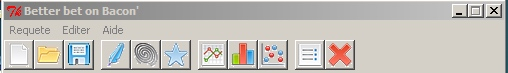
\includegraphics[scale=0.6]{barre.jpg}
\caption{Illustration de la barre d'outils}

\end{figure} 


Sur la page d’accueil, un champ libre est dédié à la réception d’une requête SQL dont nous parlerons plus loin. Un espace est également réservé à l’affichage des données.


\subsection{Connexion - Interrogation de la base de données}


En premier lieu, l'application se connectera à la base de données souhaitée. Celle-ci étant construite grâce au système PostgreSQL, le module Psycopg2 de python semble tout indiqué pour cette tâche.\\

Puis l'utilisateur disposera d'un espace dans l'interface graphique, dédié à l'insertion de la requête de son choix, celle-ci devra bien sûr être correcte ce qui demande à l’utilisateur le prérequis de la maîtrise du langage SQL.  Notre application pourra exécuter le code SQL, toujours grâce au module Psycog2.\\

La question qu’il faut se poser est comment stocker les données reçues ? Quelle structure de données allons-nous utiliser sachant qu’elle devra nous permettre de pouvoir facilement réaliser les tâches voulues à partir de ces données. Nous verrons dans la partie réalisation comment répondre à cette question.\\

Comme nous l’avons vu plus haut, il est nécessaire pour les besoins de l’utilisateur que la manipulation des requêtes soit la plus simplifiée possible, c’est pourquoi nous choisissons de mettre en place un menu déroulant « Requête » (présenté dans la partie traitant de la page d’accueil de l’IHM).\\

Pour pouvoir conserver les requêtes entre deux sessions d’exécution de Stat’nDat, nous souhaitons enregistrer ces requêtes, sous forme d’objets et les stocker dans des fichiers. C’est la raison pour laquelle nous ferons appel à une fonction de sérialisation/desérialisation pour les manipuler plus facilement. \\

Par ailleurs, le menu déroulant proposera par défaut quelques requêtes simples, de routine, qui pourront ainsi s’adapter directement à la base de données de l’utilisateur.\\

Enfin, trois boutons permettent respectivement d’effacer/annuler, valider et enregistrer la requête insérée. Cette fonction d’enregistrement de la requête est bien sûr reliée au système qui construit le menu déroulant, de manière à ce que l’on puisse retrouver sa requête directement en passant par là.


\begin{figure}[H]

\centering
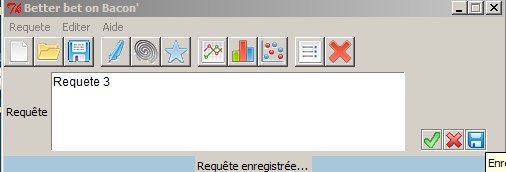
\includegraphics[scale=0.6]{requ.jpg}
\caption{Illustration de l'espace "Requête"}

\end{figure}


\subsection{Visualisation et analyse}

Les résultats seront affichés dans la deuxième partie de l'interface et dans la même fenêtre initiale, comme représenté dans la figure ci-dessous.


\begin{figure}[H]

\centering
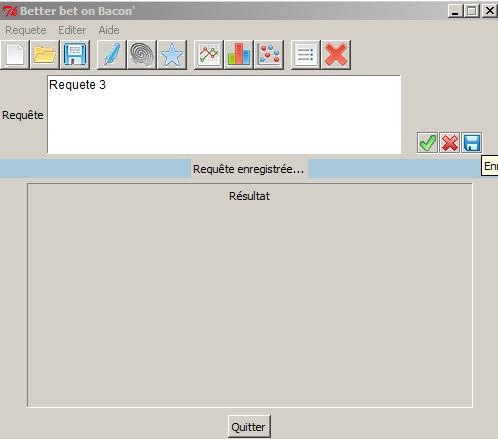
\includegraphics[scale=0.6]{res.jpg}
\caption{Illustration de l'affichage des résultats}

\end{figure}

Après affichage des résultats de la requête saisie, l'utilisateur pourra y appliquer des tests statistiques tels que les tests de Student, de Wilcoxon, ou Kruskall-Wallis. Le bilan du test effectué sera affiché dans une nouvelle fenêtre, sur laquelle sont placées des boutons correspondant aux graphiques disponibles sur l'application. L'utilisateur pourra à ce moment cliquer sur l'une des icônes pour créer un graphique qui s'affichera sur une troisième et dernière fenêtre.

\begin{figure}[H]

\centering
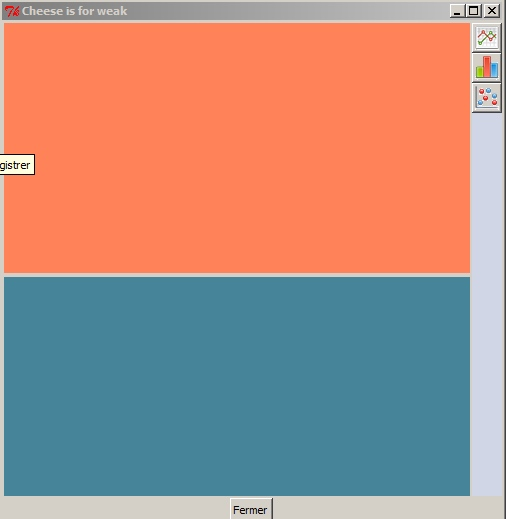
\includegraphics[scale=0.6]{test.jpg}
\caption{Illustration de l'affichage des résultats du test de Student}

\end{figure} 

L'application permet à l'utilisateur de faire une analyse  statistique des résultats obtenus des requêtes insérées. Pour effectuer les tests statistiques sur les données, l'interface graphique et les boutons décrits plus hauts permettent à l'utilisateur de lancer directement un tâche. \\

Une fois la requête lancée, le logiciel permet à l'utilisateur de visualiser ses données sous la forme d'un tableau comme décrit plus haut, c'est dans la fenêtre principale qu'un espace est spécifiquement dédié à cet usage.

La description des données, faite grâce aux différents calculs de paramètres de population est sera facultative : l'utilisateur pourra ainsi choisir s'il veut les voir apparaître ou non en fonction de ses besoins. \\
Pour cela, il lui suffira de "cocher" ou non l'option disponible dans la fenêtre de statistiques.\\

Le calcul de l'écart type, de la moyenne, et de la médiane seront faits par défaut sur tous les résultats.\\ 

L'outil donnera aussi la possibilité de créer des figures graphiques telles que les courbes, les histogrammes et les Dot-plot.\\
Des boutons permettrons à l'utilisateur de modifier directement dans la fenêtre le type de graphe. Ainsi il pourra voir successivement ses données sur plusieurs représentations différentes.\\

Grâce à Stat'nDat enfin, l'utilisateur peut générer un rapport PDF de ses résultats obtenus. L'interface lui permet de choisir la partie qui l'intéresse en ainsi générer le rapport qu'il souhaite. Pour cela, il lui suffit d'ouvrir la fenêtre dédiée à cette tâche, grâce au bouton correspondant.\\
Le rapport contiendra aussi bien les différents graphiques de représentation des données que les résultats chiffrés des tests paramétriques ou non. Enfin, et c'est le plus important, pour éviter à l'utilisateur de rédiger plusieurs fois le même "squelette" textuel, les paragraphes seront déjà présents et s'adaptent directement aux données obtenues. C'est ce qui permet l'automatisation de la tâche.


\subsection{Modifications internes}

Notre architecture logicielle comprend :

\begin{itemize}

\item • Un fichier pour gérer la partie "connexion et interrogation de la base de données".

\item • Un fichier pour gérer la partie "interface graphique".

\item • Un fichier pour gérer la partie "statistiques".

\item • Un fichier pour gérer la partie "génération du rapport PDF".

\item • Un fichier qui fera la liaison entre les quatre fichiers précédents et qui servira donc d'exécutable.

\end{itemize}


Grâce à cela, l'ajout d'un test statistique pourra se faire en passant par le code. Le module Statistique le permet, il suffit d'ajouter une fonction dans le code.
Ce simple ajout et nous nous verrons plus précisément comment dans la partie réalisation, devra suffire à ce que le test ajouté soit pris en compte dans l'interface graphique et dans la rédaction du rapport PDF.


\chapter{Réalisation}


\chapter*{Conclusion}

\addcontentsline{toc}{section}{Conclusion}

 \end{document}  